\documentclass{beamer}
\usepackage[utf8]{inputenc}
\usepackage{tikz}
\usetikzlibrary{shapes, arrows, mindmap, positioning, chains, shadows, backgrounds}
\usetikzlibrary{shapes.geometric, arrows, positioning}
\usepackage{pgfplots}
\usepackage{graphicx}
% Definición de un estilo para los bloques de contenido
\useinnertheme{rounded}
%\useoutertheme{sidebar}
\setbeamertemplate{navigation symbols}{}

% Paleta de colores (opcional, para un diseño más atractivo)
\definecolor{mitblue}{RGB}{0, 64, 128}
\definecolor{mitgray}{RGB}{169, 169, 169}
\setbeamercolor{palette primary}{bg=mitblue, fg=white}
\setbeamercolor{palette secondary}{bg=mitblue, fg=white}
\setbeamercolor{palette tertiary}{bg=mitblue, fg=white}
\setbeamercolor{title}{bg=mitblue, fg=white}
\setbeamercolor{frametitle}{bg=mitblue, fg=white}
\setbeamercolor{block title}{bg=mitblue!80!black, fg=white}
\setbeamercolor{block body}{bg=mitgray!20!white}
\setbeamercolor{sidebar}{bg=mitblue}


\title{Introducción a la Inteligencia Artificial}
\author{Sergio Hernández.\\ PhD Computer Science}
\institute{Magister en Data Science. Universidad Católica del Maule}
%\date{\today}

\begin{document}

% --- Diapositiva de Título ---
\begin{frame}
  \titlepage
\end{frame}

% --- Diapositiva 1: ¿Qué es la IA? ---
\begin{frame}{¿Qué es la Inteligencia Artificial?}
  \begin{block}{Definición Conceptual}
    La Inteligencia Artificial (IA) es una rama de la informática dedicada a la creación de agentes inteligentes, que son sistemas que pueden razonar, aprender y actuar de forma autónoma.
    \vspace{0.5cm}
    
    \textit{"Es la ciencia e ingeniería de hacer máquinas inteligentes, especialmente programas de ordenador inteligentes."} - John McCarthy, 1956.
  \end{block}
  

\end{frame}

\begin{frame}{¿Qué es la Inteligencia Artificial?}
\begin{columns}[T]
   \begin{column}{.5\textwidth}
        \begin{block}{Tipos de IA}
          \begin{itemize}
      \item \textbf{Inteligencia Artificial (IA):} El concepto global de máquinas que imitan la inteligencia humana.
      \item \textbf{Aprendizaje Automático (Machine Learning - ML):} Un subcampo de la IA donde las máquinas aprenden de los datos.
      \item \textbf{Aprendizaje Profundo (Deep Learning - DL):} Un subcampo del ML basado en redes neuronales con múltiples capas.
  \end{itemize}
        \end{block}
    \end{column}
    \begin{column}{.5\textwidth}
        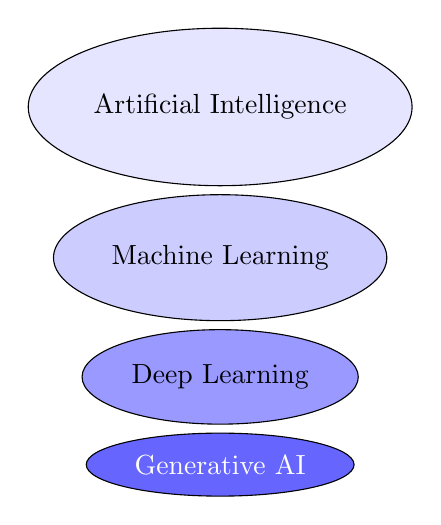
\begin{tikzpicture}
\tikzstyle{level 1}=[shape=ellipse, draw=black, fill=blue!10, minimum width=4cm, minimum height=2cm, text centered]
\tikzstyle{level 2}=[shape=ellipse, draw=black, fill=blue!20, minimum width=3.2cm, minimum height=1.6cm, text centered]
\tikzstyle{level 3}=[shape=ellipse, draw=black, fill=blue!40, minimum width=2.4cm, minimum height=1.2cm, text centered]
\tikzstyle{level 4}=[shape=ellipse, draw=black, fill=blue!60, minimum width=1.6cm, minimum height=0.8cm, text centered, text=white]

\node (ai) [level 1] {Artificial Intelligence};
\node (ml) [level 2, below=0.1cm of ai] {Machine Learning};
\node (dl) [level 3, below=0.1cm of ml] {Deep Learning};
\node (genai) [level 4, below=0.1cm of dl] {Generative AI};
\end{tikzpicture}
    \end{column}
  \end{columns}

  

\end{frame}

% --- Diapositiva 2: Un Poco de Historia ---
\begin{frame}{Un poco de historia}
\begin{itemize}
\item Década de 1950: Nace la IA como disciplina formal en el Dartmouth Workshop (1956).
\item Décadas de 1960-1970: Optimismo inicial y el "invierno de la IA".
\item Décadas de 1980-1990: Auge de los sistemas expertos y el renacimiento de las redes neuronales.
\item Década de 2000-Presente: Big Data, hardware más potente y avances en el Deep Learning impulsan la IA a un nuevo nivel.
\end{itemize}
\end{frame}

\begin{frame}{Inviernos de la IA}
  
  \begin{columns}[T]
    \begin{column}{.5\textwidth}
        \begin{block}{Épocas de Optimismo}
            \itemize{
                \item \textbf{Años 50-70:} Fundación, lógica simbólica y grandes promesas.
                \item \textbf{Años 80:} Auge de los sistemas expertos en la industria.
                \item \textbf{Años 2010-Hoy:} La era del Big Data, GPUs y Deep Learning.
            }
        \end{block}
    \end{column}
    \begin{column}{.5\textwidth}
        \begin{block}{Los "Inviernos" de la IA}
            \itemize{
                \item Períodos de recortes de financiación y pérdida de interés.
                \item Causados por promesas excesivas y limitaciones computacionales.
                \item \textbf{Lección clave:} La importancia de gestionar las expectativas.
            }
        \end{block}
    \end{column}
  \end{columns}
\end{frame}

% --- Diapositiva 3: Tipos de IA ---
\begin{frame}{Tipos de IA: IA Débil vs. IA Fuerte (AGI)}
  \begin{columns}[T]
    \begin{column}{.5\textwidth}
        \begin{block}{IA Débil (Narrow AI)}
            \begin{itemize}
                \item Es la IA que tenemos hoy.
                \item Diseñada y entrenada para una \textbf{tarea específica}.
                \item Ejemplos: Reconocimiento facial, asistentes de voz, sistemas de recomendación.
                \item No posee conciencia ni entendimiento real.
            \end{itemize}
        \end{block}
    \end{column}
    \begin{column}{.5\textwidth}
        \begin{block}{IA Fuerte / General (AGI)}
            \begin{itemize}
                \item Inteligencia a nivel humano.
                \item Capaz de entender, aprender y aplicar su inteligencia para resolver \textbf{cualquier problema}.
                \item Es el objetivo (aún lejano) de la investigación en IA.
                \item Plantea enormes debates filosóficos y éticos.
            \end{itemize}
        \end{block}
    \end{column}
  \end{columns}
  
  \begin{center}
  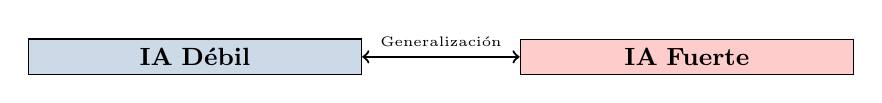
\begin{tikzpicture}[node distance=2cm, auto, font=\small]
    \node (narrow) [rectangle, draw, fill=mitblue!20, text width=4cm, align=center] { \textbf{IA Débil}};
    \node (agi) [rectangle, draw, fill=red!20, text width=4cm, align=center, right=of narrow] { \textbf{IA Fuerte }};
    \draw[<->, thick] (narrow) -- (agi) node[midway, above,font=\tiny] {Generalización};
  \end{tikzpicture}
  \end{center}
\end{frame}


% --- Diapositiva 4: La Prueba de Turing ---
\begin{frame}{La Prueba de Turing: ¿Pueden pensar las máquinas?}
  Propuesta por Alan Turing en 1950 como una forma de evaluar la inteligencia de una máquina.
  
  \begin{block}{El Juego de la Imitación}
    Un interrogador humano (C) se comunica por texto con un humano (B) y una máquina (A). Si el interrogador no puede distinguir consistentemente cuál es la máquina, se dice que la máquina ha pasado la prueba.
  \end{block}
  
  \begin{center}
  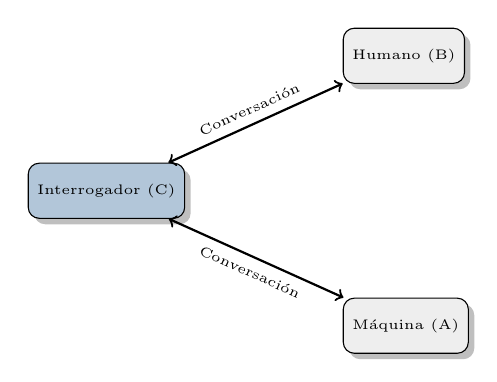
\begin{tikzpicture}[
    node/.style={rectangle, draw, fill=mitgray!20, rounded corners, minimum height=0.7cm, minimum width=1cm, drop shadow},
    font=\tiny
  ]
    \node (interrogador) [node, fill=mitblue!30] {Interrogador (C)};
    \node (humano) [node, above right=1cm and 2cm of interrogador] {Humano (B)};
    \node (maquina) [node, below right=1cm and 2cm of interrogador] {Máquina (A)};
    \draw[<->, thick] (interrogador) -- (humano) node[midway, above, sloped] {Conversación};
    \draw[<->, thick] (interrogador) -- (maquina) node[midway, below, sloped] {Conversación};
    
    
  \end{tikzpicture}
  \end{center}


\end{frame}

% --- Diapositiva 5: Enfoques Principales de la IA ---
\begin{frame}{Enfoques Principales: Símbolos vs. Conexiones}
  Históricamente, la IA ha seguido dos grandes filosofías:
  
  \begin{columns}[T]
    \begin{column}{.5\textwidth}
        \begin{block}{IA Simbólica (Top-Down)}
            \begin{itemize}
                \item \textbf{Idea:} La inteligencia se puede lograr mediante la manipulación de símbolos y reglas lógicas.
                \item \textbf{Método:} Representar el conocimiento explícitamente en una base de conocimiento y usar un motor de inferencia.
                \item \textbf{Ejemplo: %$SI (fiebre > 38 \wedge tos = seca) \implies (diagnostico = posible_gripe)$ 
                \texttt{SI (fiebre > 38 Y tos = seca) ENTONCES (diagnostico = gripe)} 
                }
               \end{itemize}
        \end{block}
    \end{column}
    \begin{column}{.5\textwidth}
        \begin{block}{IA Conexionista (Bottom-Up)}
            \begin{itemize}
                \item \textbf{Idea:} La inteligencia emerge de la interconexión de muchas unidades simples (neuronas).
                \item \textbf{Método:} Aprender patrones y representaciones directamente de los datos, sin reglas explícitas.
                \item \textbf{Ejemplo:} Redes Neuronales Artificiales.
            \end{itemize}
        \end{block}
    \end{column}
  \end{columns}
\end{frame}
%
%% --- Diapositiva 6: El Auge del Aprendizaje Automático ---
\begin{frame}{Aprendizaje Automático}
  El enfoque conexionista evolucionó hacia el Machine Learning, que es el motor de la IA moderna.

  \begin{center}
  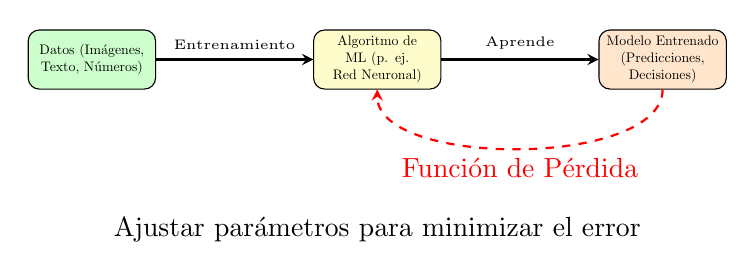
\begin{tikzpicture}[
    node/.style={rectangle, draw, fill=mitblue!20, rounded corners, text width=3cm, align=center, minimum height=1.5cm,scale=0.5},
    arrow/.style={->, >=stealth, thick}
  ]
    \node (datos) [node, fill=green!20] {Datos  (Imágenes, Texto, Números)};
    \node (modelo) [node, fill=yellow!20, right=2cm of datos] {Algoritmo de ML  (p. ej. Red Neuronal)};
    \node (prediccion) [node, fill=orange!20, right=2cm of modelo] {Modelo Entrenado  (Predicciones, Decisiones)};
    
    \draw[arrow] (datos) -- (modelo) node[midway, above,font=\tiny] {Entrenamiento};
    \draw[arrow] (modelo) -- (prediccion) node[midway, above,font=\tiny] {Aprende};
    
    \node (feedback) [below=1.5cm of modelo] {Ajustar parámetros para minimizar el error};
    \draw[arrow, dashed, red] (prediccion.south) .. controls +(south:1cm) and +(south:1cm) .. (modelo.south) node[midway, below, align=center] {Función de  Pérdida};
  \end{tikzpicture}
  \end{center}
  
  \begin{block}{Paradigmas}
    \begin{itemize}
        \item \textbf{Supervisado:} Aprender de datos etiquetados (p. ej. imágenes de gatos con la etiqueta "gato").
        \item \textbf{No Supervisado:} Encontrar estructura en datos no etiquetados (p. ej. agrupar clientes por comportamiento).
        \item \textbf{Por Refuerzo:} Aprender a través de prueba y error, con recompensas y castigos 
    \end{itemize}
  \end{block}
\end{frame}
%
%% --- Diapositiva 7: Ecosistema de la IA ---
\begin{frame}{El Ecosistema de la IA}
    
    \begin{center}
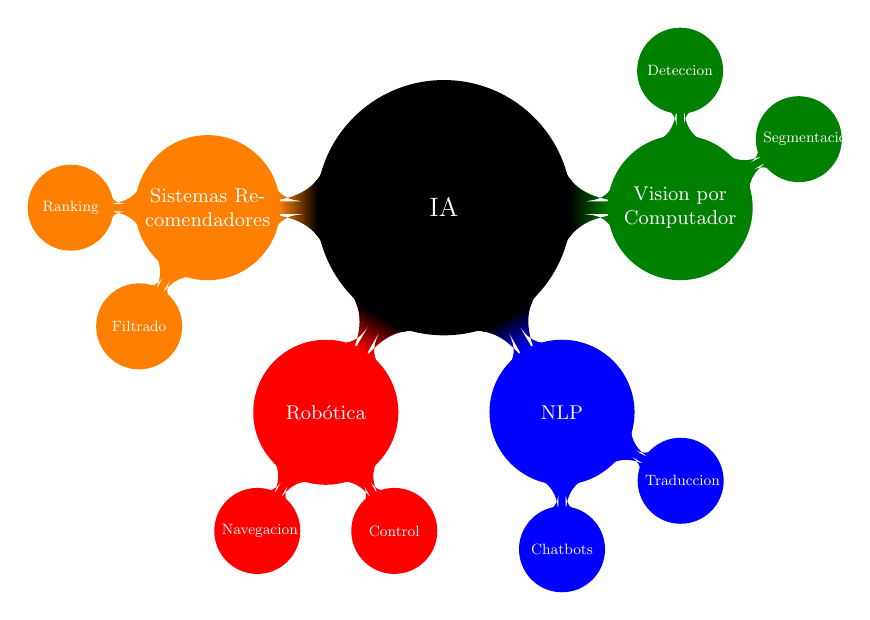
\begin{tikzpicture}[scale=0.6]
  \path[mindmap,concept color=black,text=white]
    node[concept,scale=0.8,level distance = 20mm] {IA}
    [clockwise from=0]
    % note that `sibling angle' can only be defined in
    % `level 1 concept/.append style={}'
    child[concept color=green!50!black] {
      node[concept,scale=0.8,font=\small] {Vision por Computador}
      [clockwise from=90]
      child { node[concept,scale=0.6,font=\small] {Deteccion} }
      child { node[concept,scale=0.6,font=\small] {Segmentacion} }
    }
    % note that the `concept color' is passed to the `child'(!)
    child[concept color=blue] {
      node[concept,scale=0.8,font=\small] {NLP}
      [clockwise from=-30]
      child { node[concept,scale=0.6,font=\small] {Traduccion} }
      child { node[concept,scale=0.6,font=\small] {Chatbots} }
    }
     child[concept color=red] {
      node[concept,scale=0.8,font=\small] {Robótica}
      [clockwise from=-60]
      child { node[concept,scale=0.6,font=\small] {Control} }
      child { node[concept,scale=0.6,font=\small] {Navegacion} }
    }
    child[concept color=orange] {
      node[concept,scale=0.8,font=\small] {Sistemas Recomendadores}
      [clockwise from=-120]
      child { node[concept,scale=0.6,font=\small] {Filtrado} }
      child { node[concept,scale=0.6,font=\small] {Ranking} }
    };
\end{tikzpicture}
    \end{center}
\end{frame}

\begin{frame}{Deep Learning (Aprendizaje Profundo)}
\begin{columns}[T]
   \begin{column}{.5\textwidth}
        \begin{block}{Paridad Humana}
          \begin{itemize}
      \item \textbf{2015} Clasificación de Imágenes.
      \item \textbf{2016} Reconocimiento del Habla
      \item \textbf{2018} Traducción Automática.
       \item \textbf{2020} Subtítulos en Imágenes
  \end{itemize}
        \end{block}
    \end{column}
    \begin{column}{.5\textwidth}
    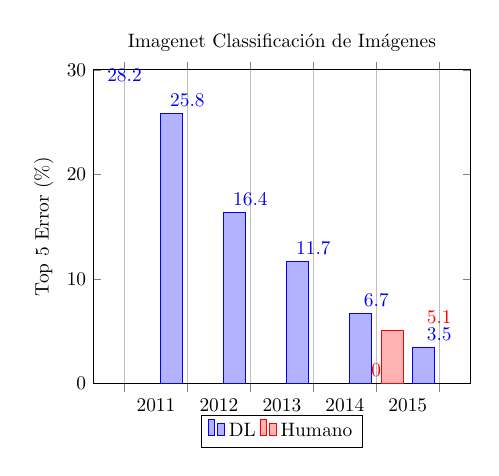
\begin{tikzpicture}[scale=0.7]
\begin{axis}[
       title={Imagenet Classificación de Imágenes},
	x tick label style={
		/pgf/number format/1000 sep=},
	ylabel=Top 5 Error (\%),
	 bar width=0.4cm,
        ymin=0, ymax=30,
	legend style={at={(0.5,-0.1)},
	anchor=north,legend columns=-1},
	ybar interval=0.7,
	symbolic x coords={
           2010,2011,2012,2013,2014,2015},
          xtick=data,
          nodes near coords={
        \pgfmathprintnumber[precision=1]{\pgfplotspointmeta}
       }
]
\addplot 
	coordinates {(2015,3.5) (2014,6.7)
		 (2013,11.7) (2012,16.4) (2011,25.8) (2010,28.2)};
\addplot 
	coordinates {(2015,5.1) (2014,0)};
\legend{DL,Humano}
\end{axis}
\end{tikzpicture}
     \end{column}
  \end{columns}
  \end{frame}

\begin{frame}{IA Generativa}
% TODO: \usepackage{graphicx} required
\begin{figure}
	\centering
	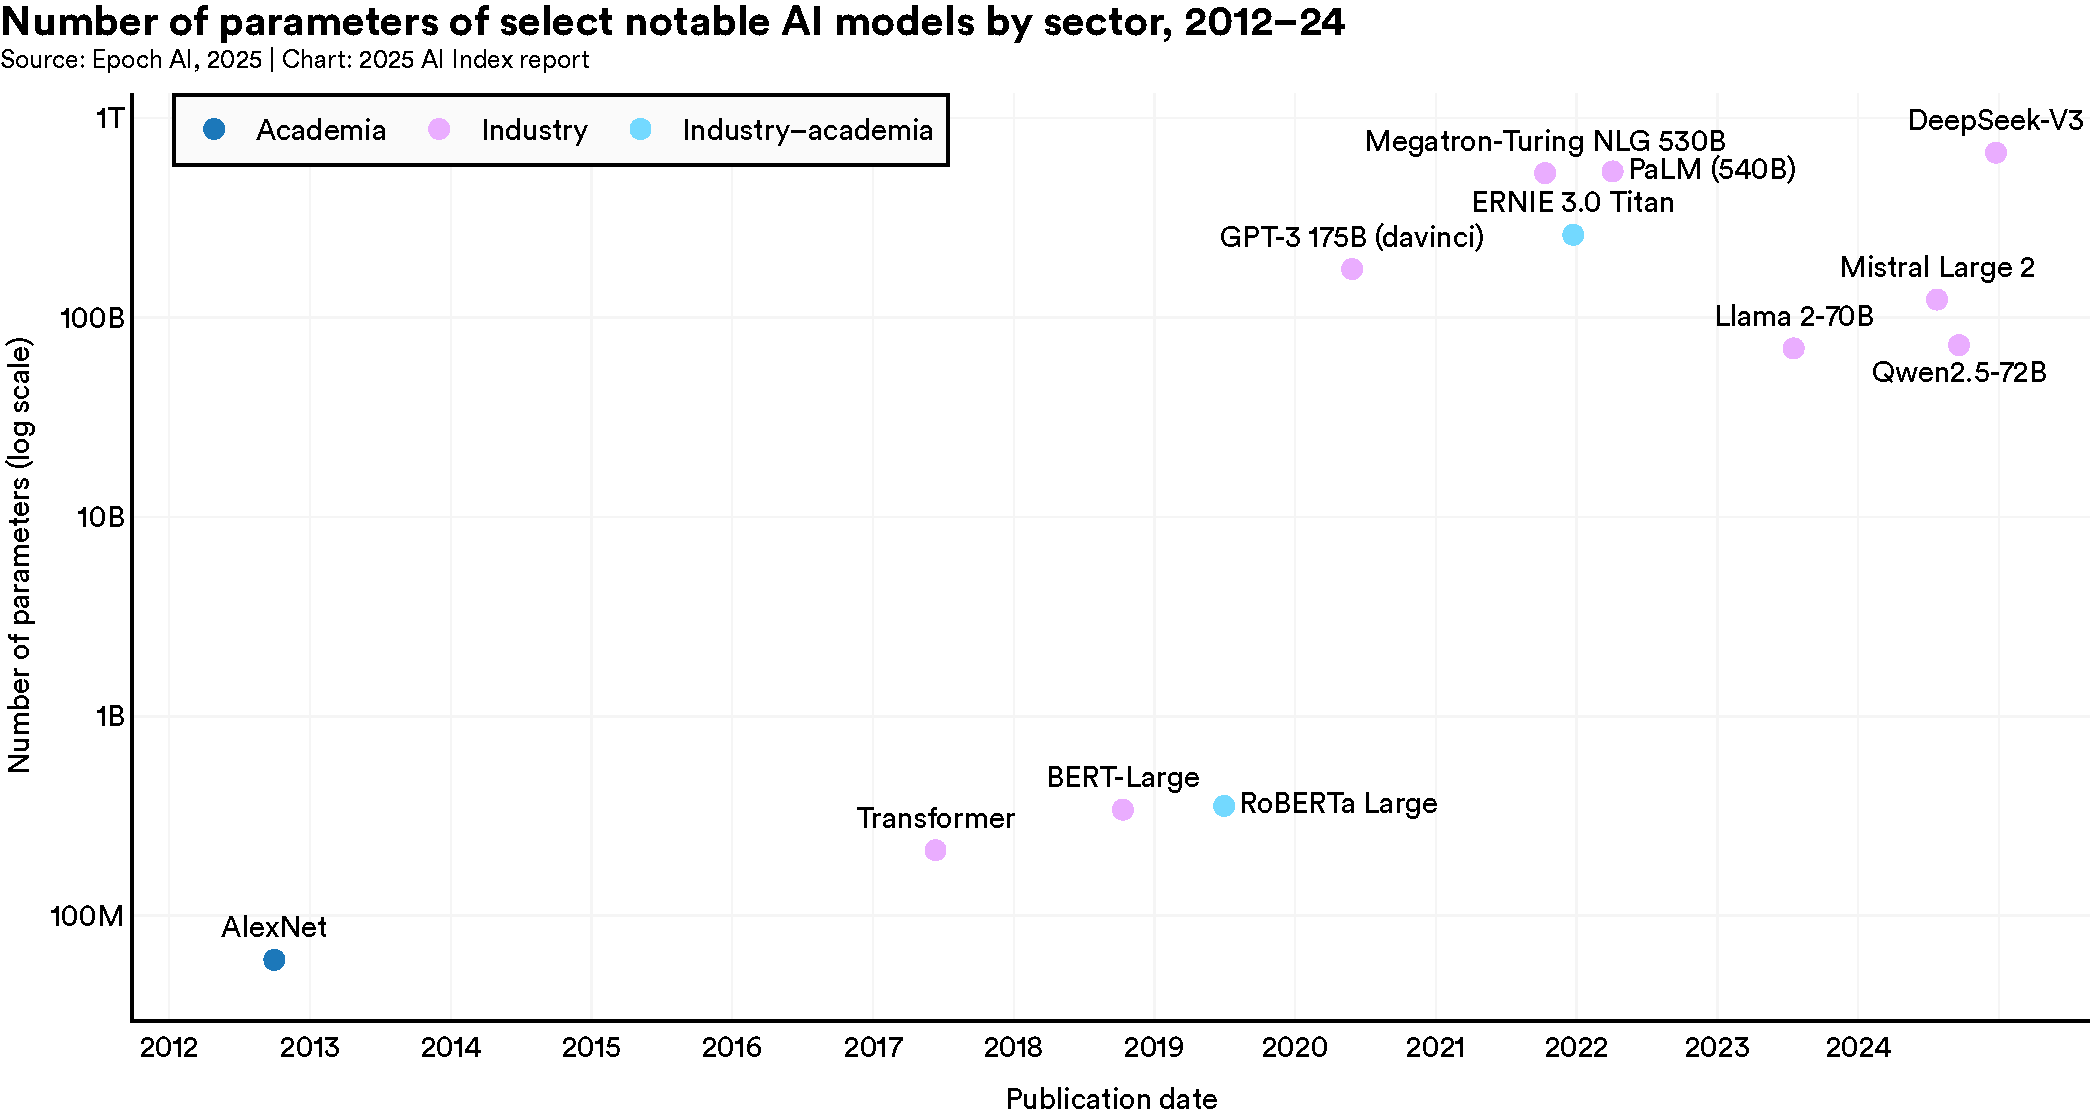
\includegraphics[width=\linewidth]{figures/fig_1.3.12}
	\caption{AI Index Report \url{https://hai.stanford.edu/ai-index/2025-ai-index-report}}
	\label{fig:fig1}
\end{figure}


  \end{frame}


\begin{frame}{Bases de Datos}
\begin{figure}
	\centering
	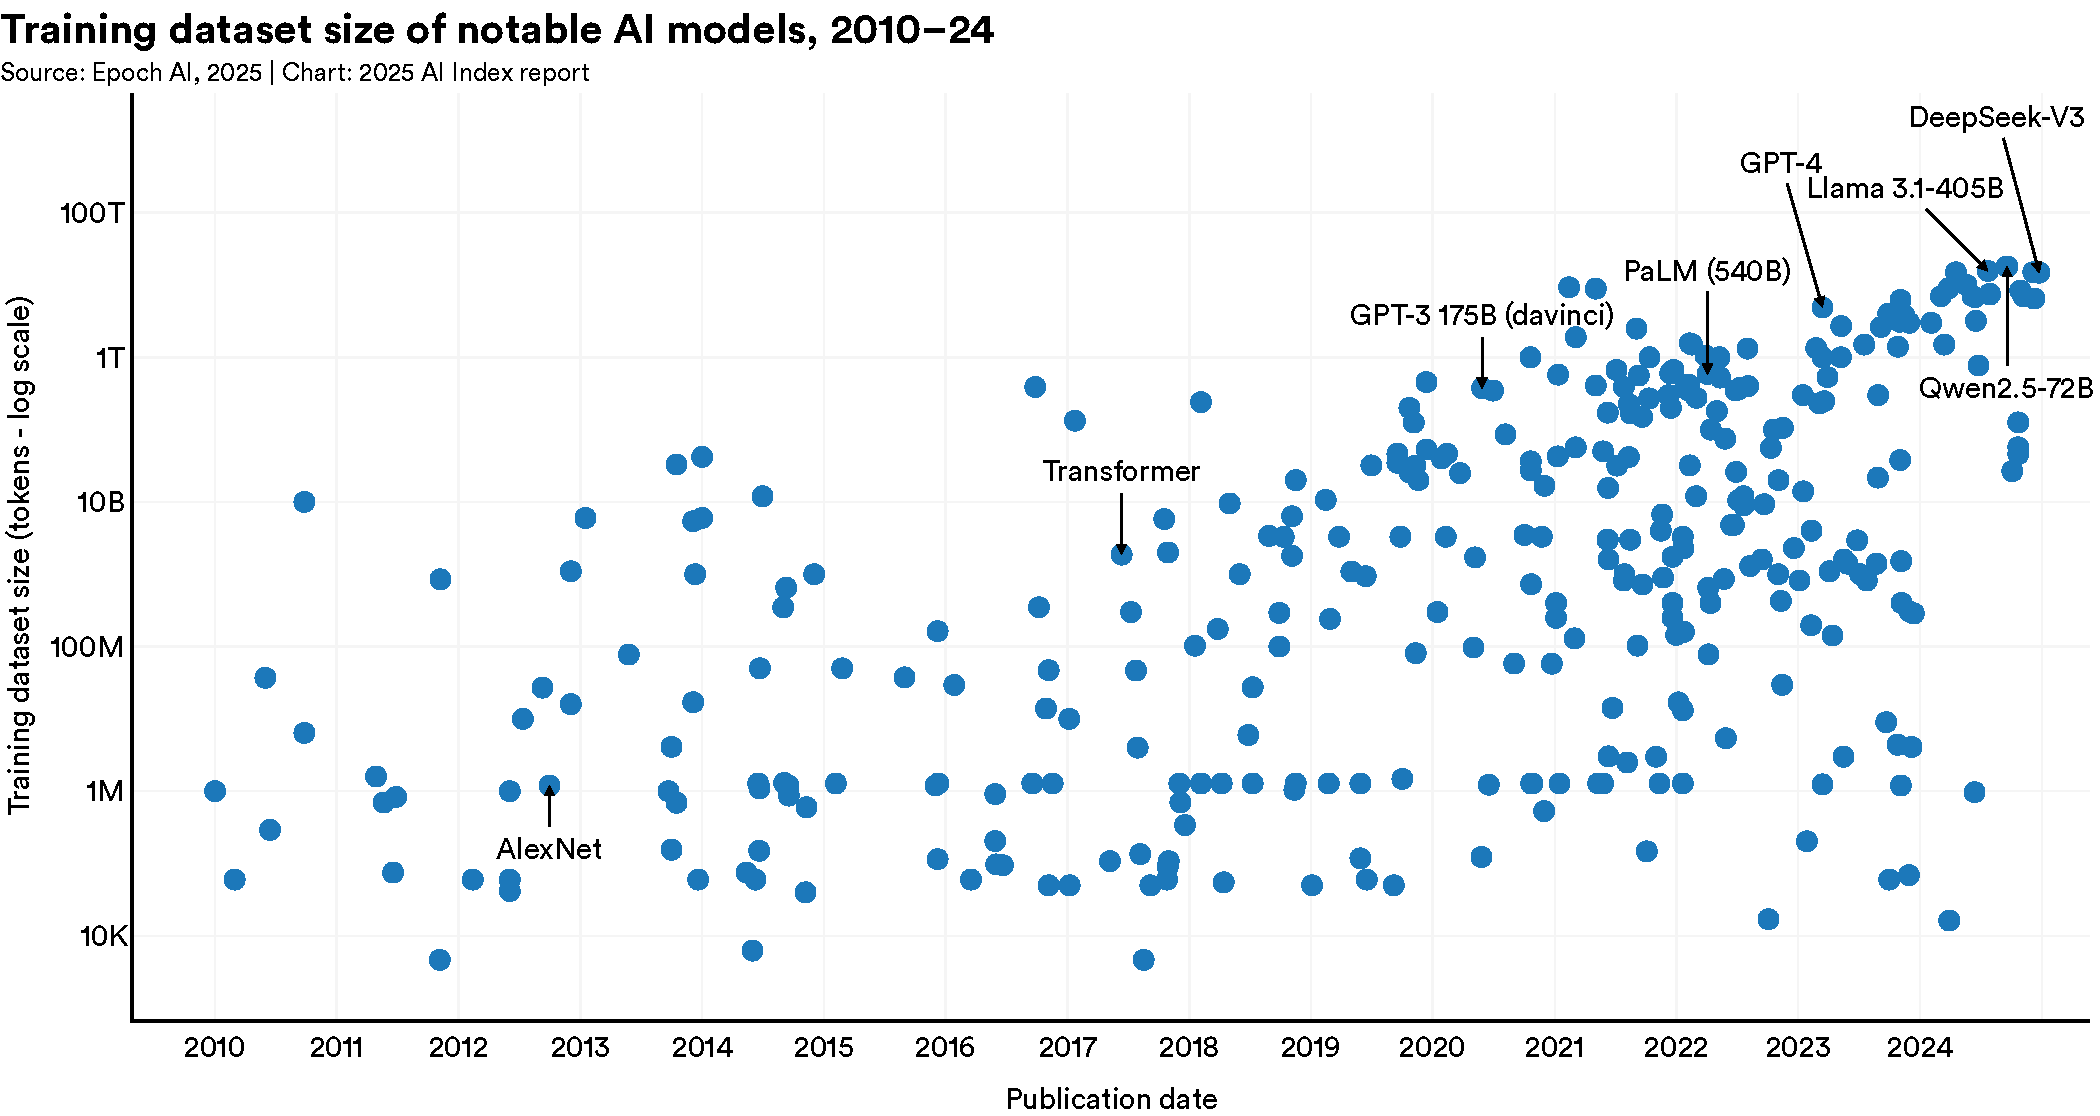
\includegraphics[width=\linewidth]{figures/fig_1.3.13}
	\caption{AI Index Report \url{https://hai.stanford.edu/ai-index/2025-ai-index-report}}
	\label{fig:fig2}
\end{figure}
\end{frame}

\begin{frame}{Huella de Carbono}
	\begin{figure}
		\centering
		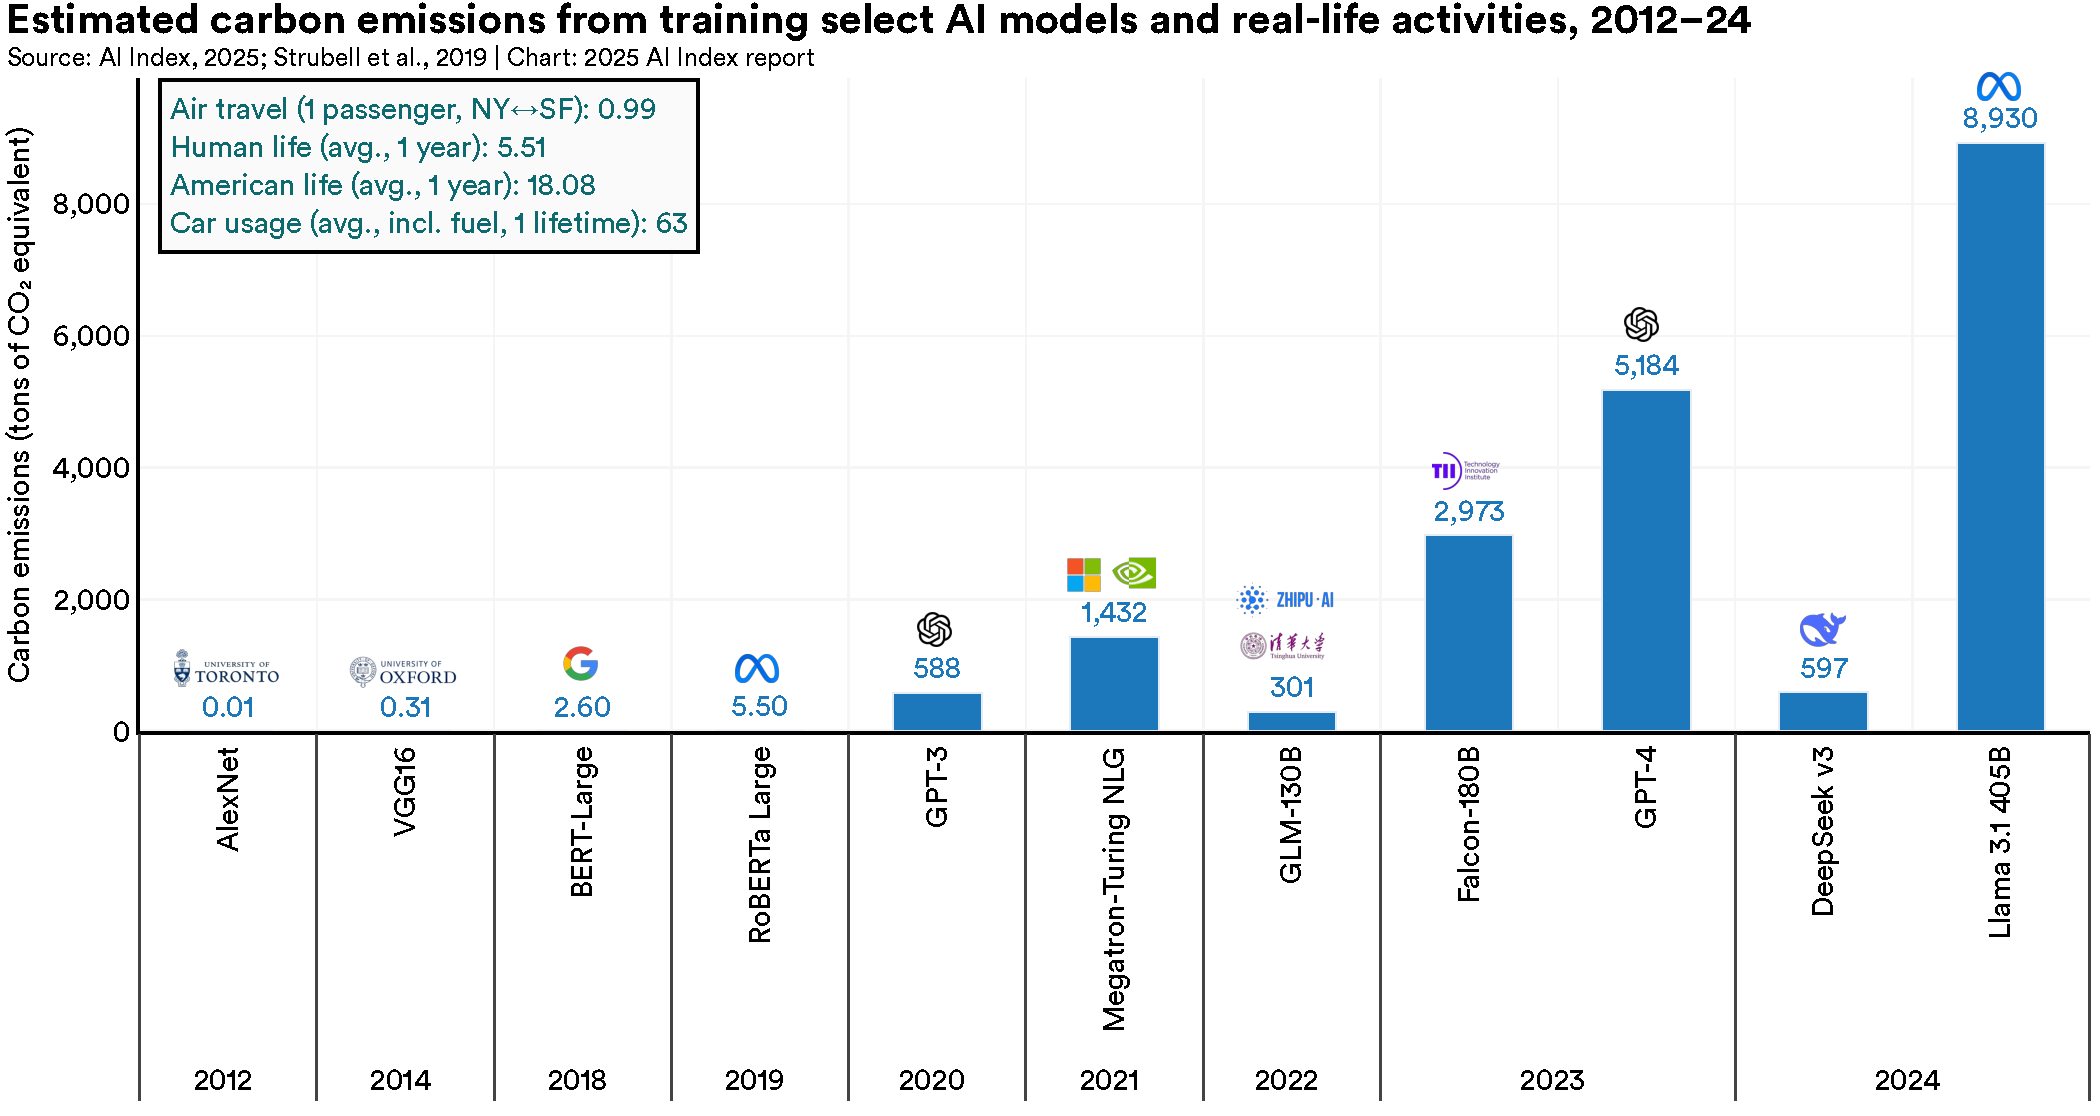
\includegraphics[width=\linewidth]{figures/fig_1.4.7}
		\caption{AI Index Report \url{https://hai.stanford.edu/ai-index/2025-ai-index-report}}
		\label{fig:fig3}
	\end{figure}
\end{frame}

\begin{frame}{Performance}
	\begin{figure}
		\centering
		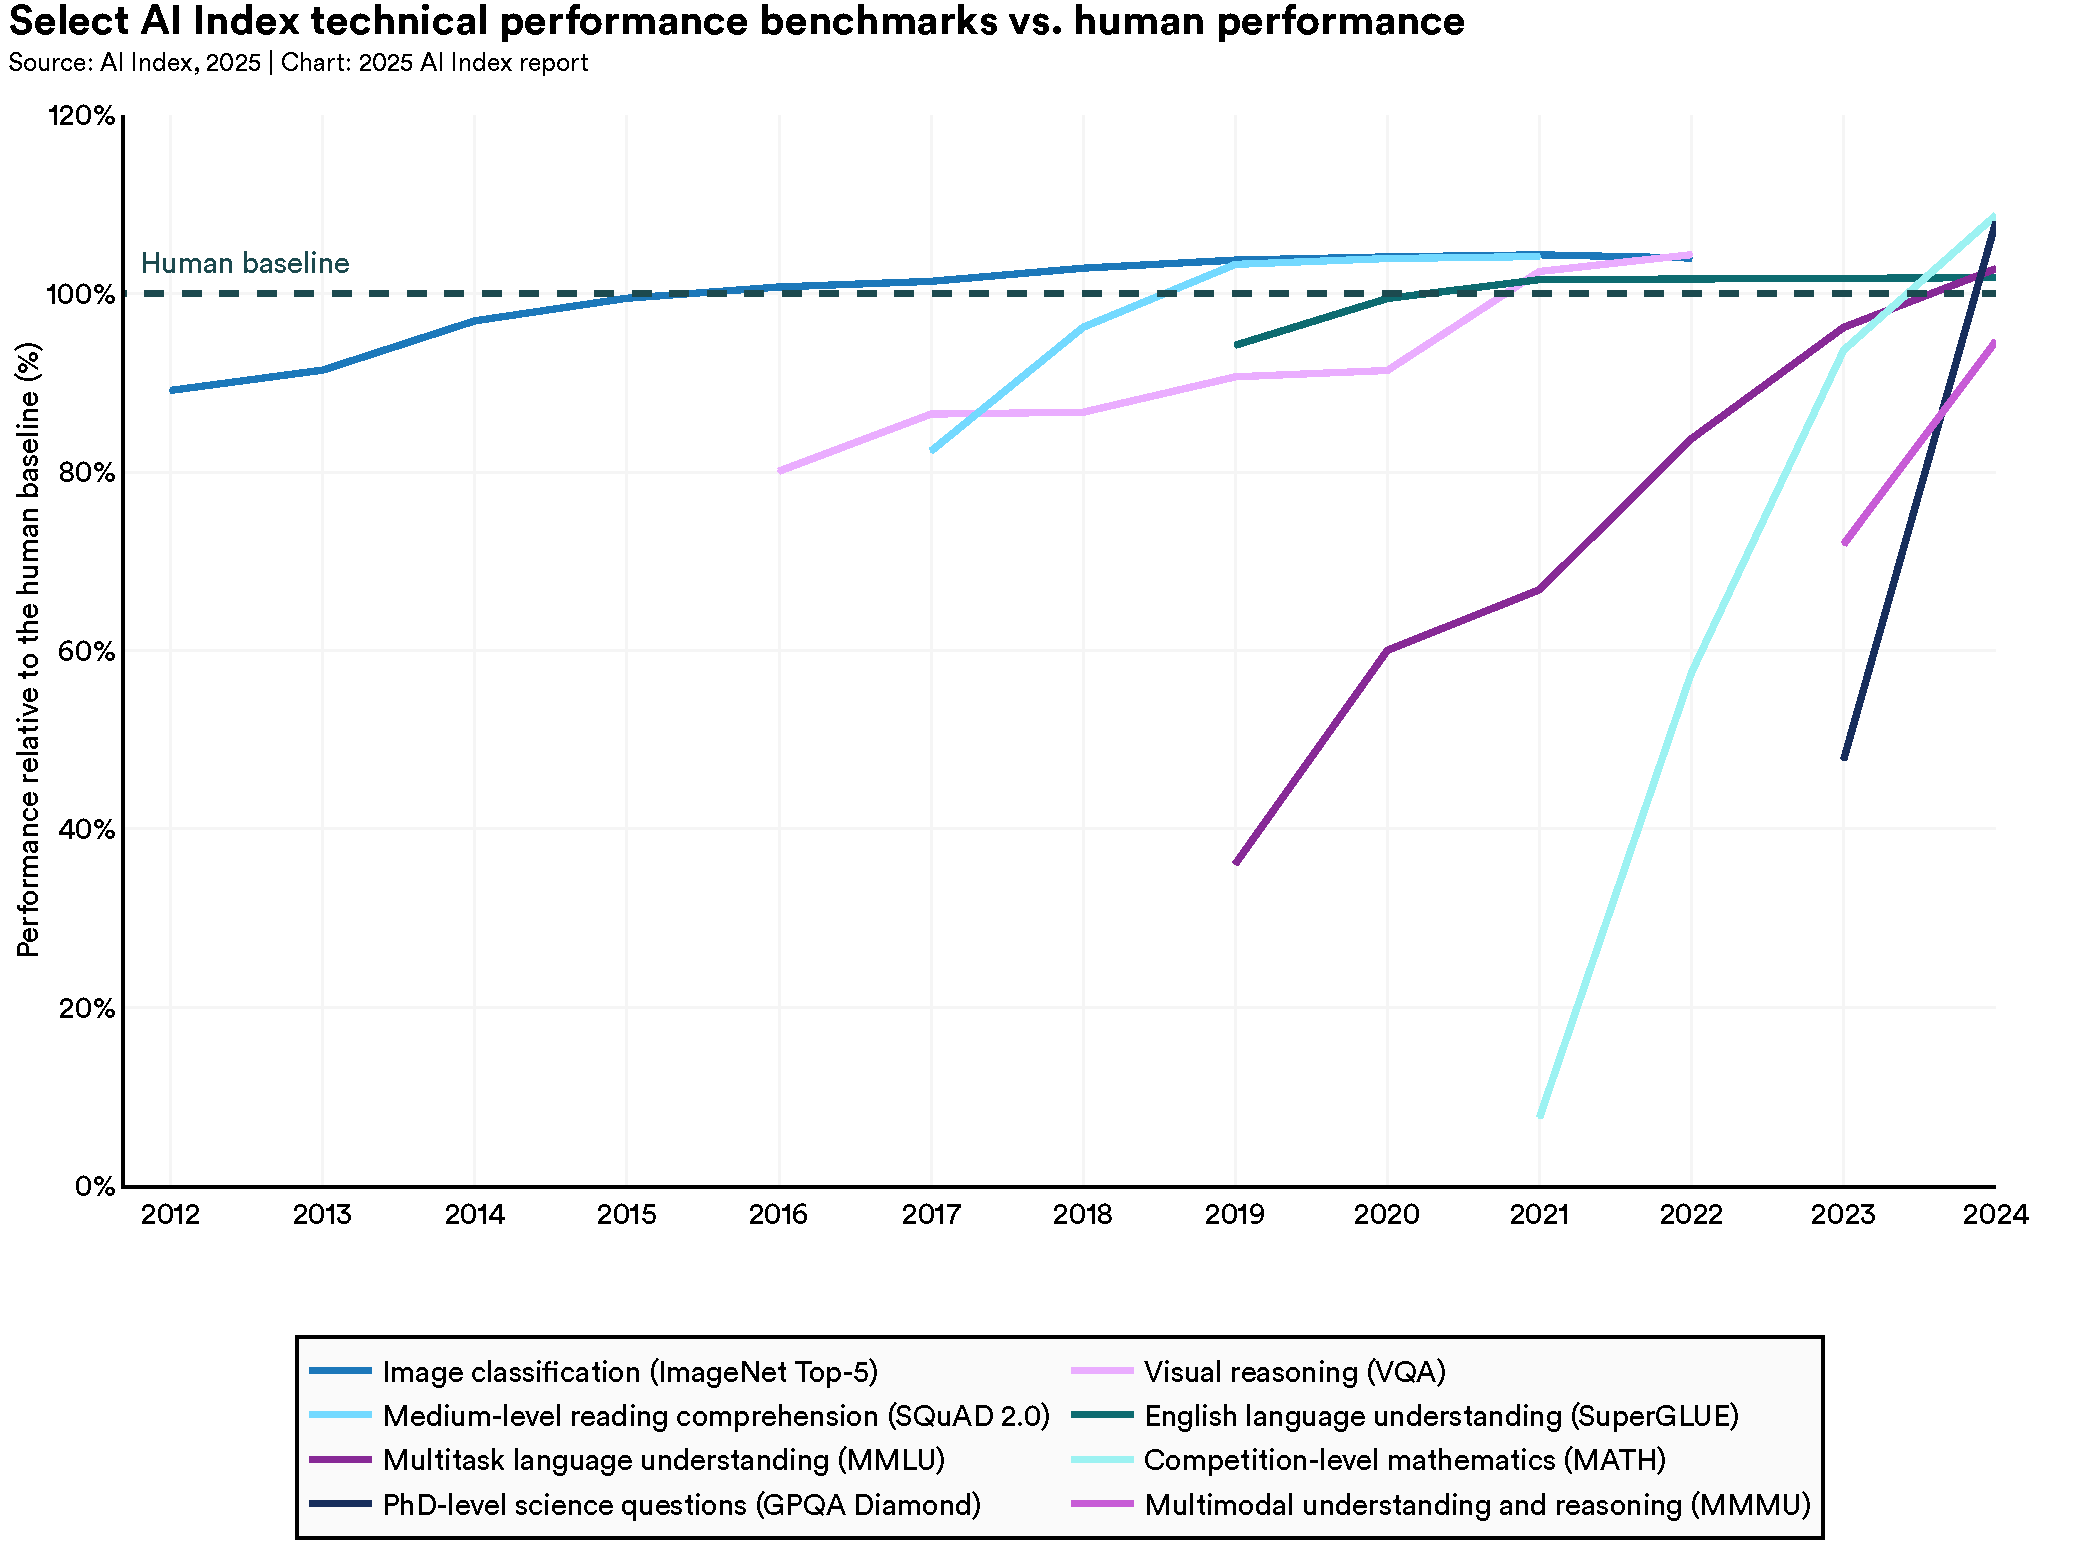
\includegraphics[width=\linewidth]{figures/fig_2.1.33}
		\caption{AI Index Report \url{https://hai.stanford.edu/ai-index/2025-ai-index-report}}
		\label{fig:fig4}
	\end{figure}
\end{frame}

\begin{frame}{Comprensión (Massive Multitask Language Understanding)}
	\begin{figure}
		\centering
		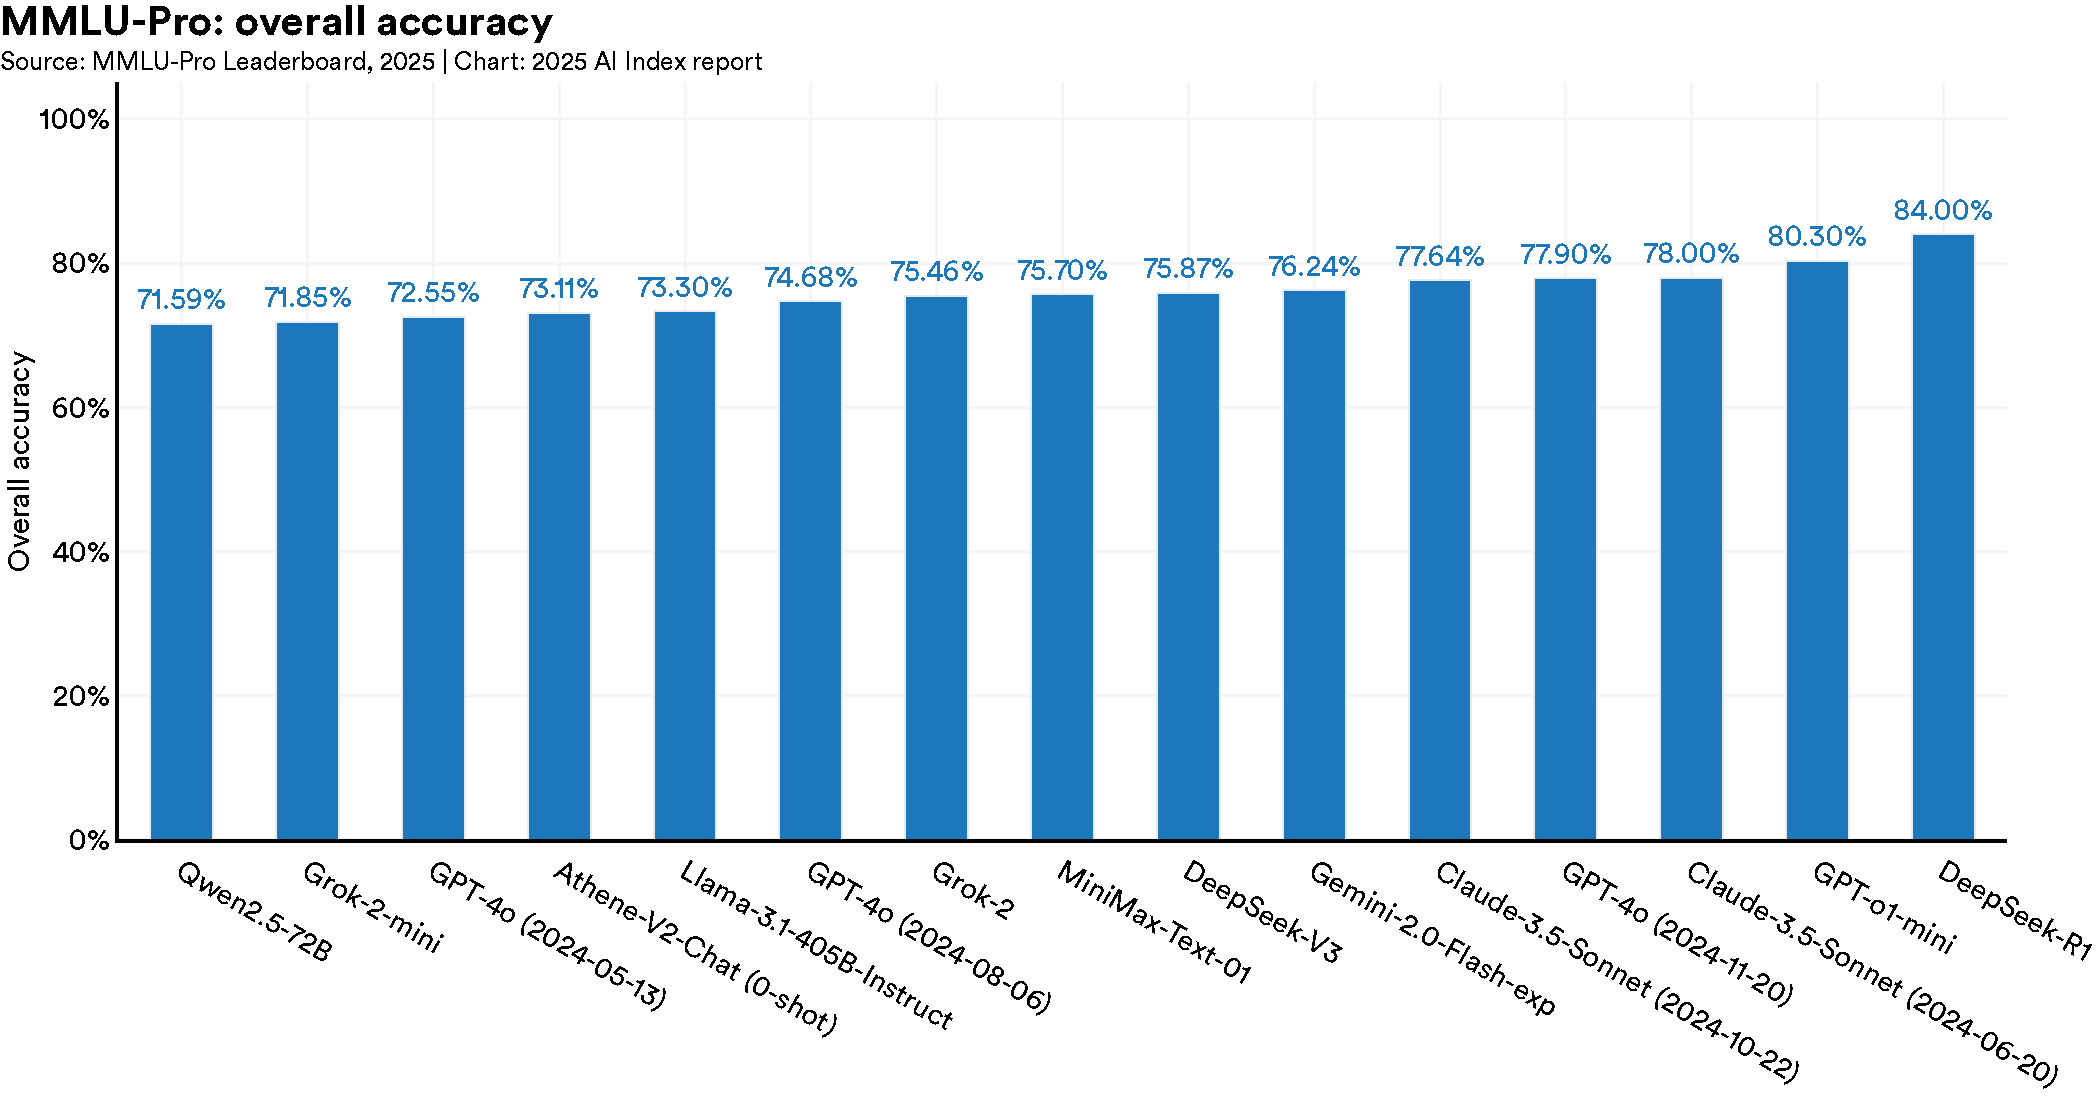
\includegraphics[width=\linewidth]{figures/fig_2.2.5}
		\caption{AI Index Report \url{https://hai.stanford.edu/ai-index/2025-ai-index-report}}
		\label{fig:fig5}
	\end{figure}
\end{frame}

\begin{frame}{Resolución de Problemas}
	\begin{figure}
		\centering
		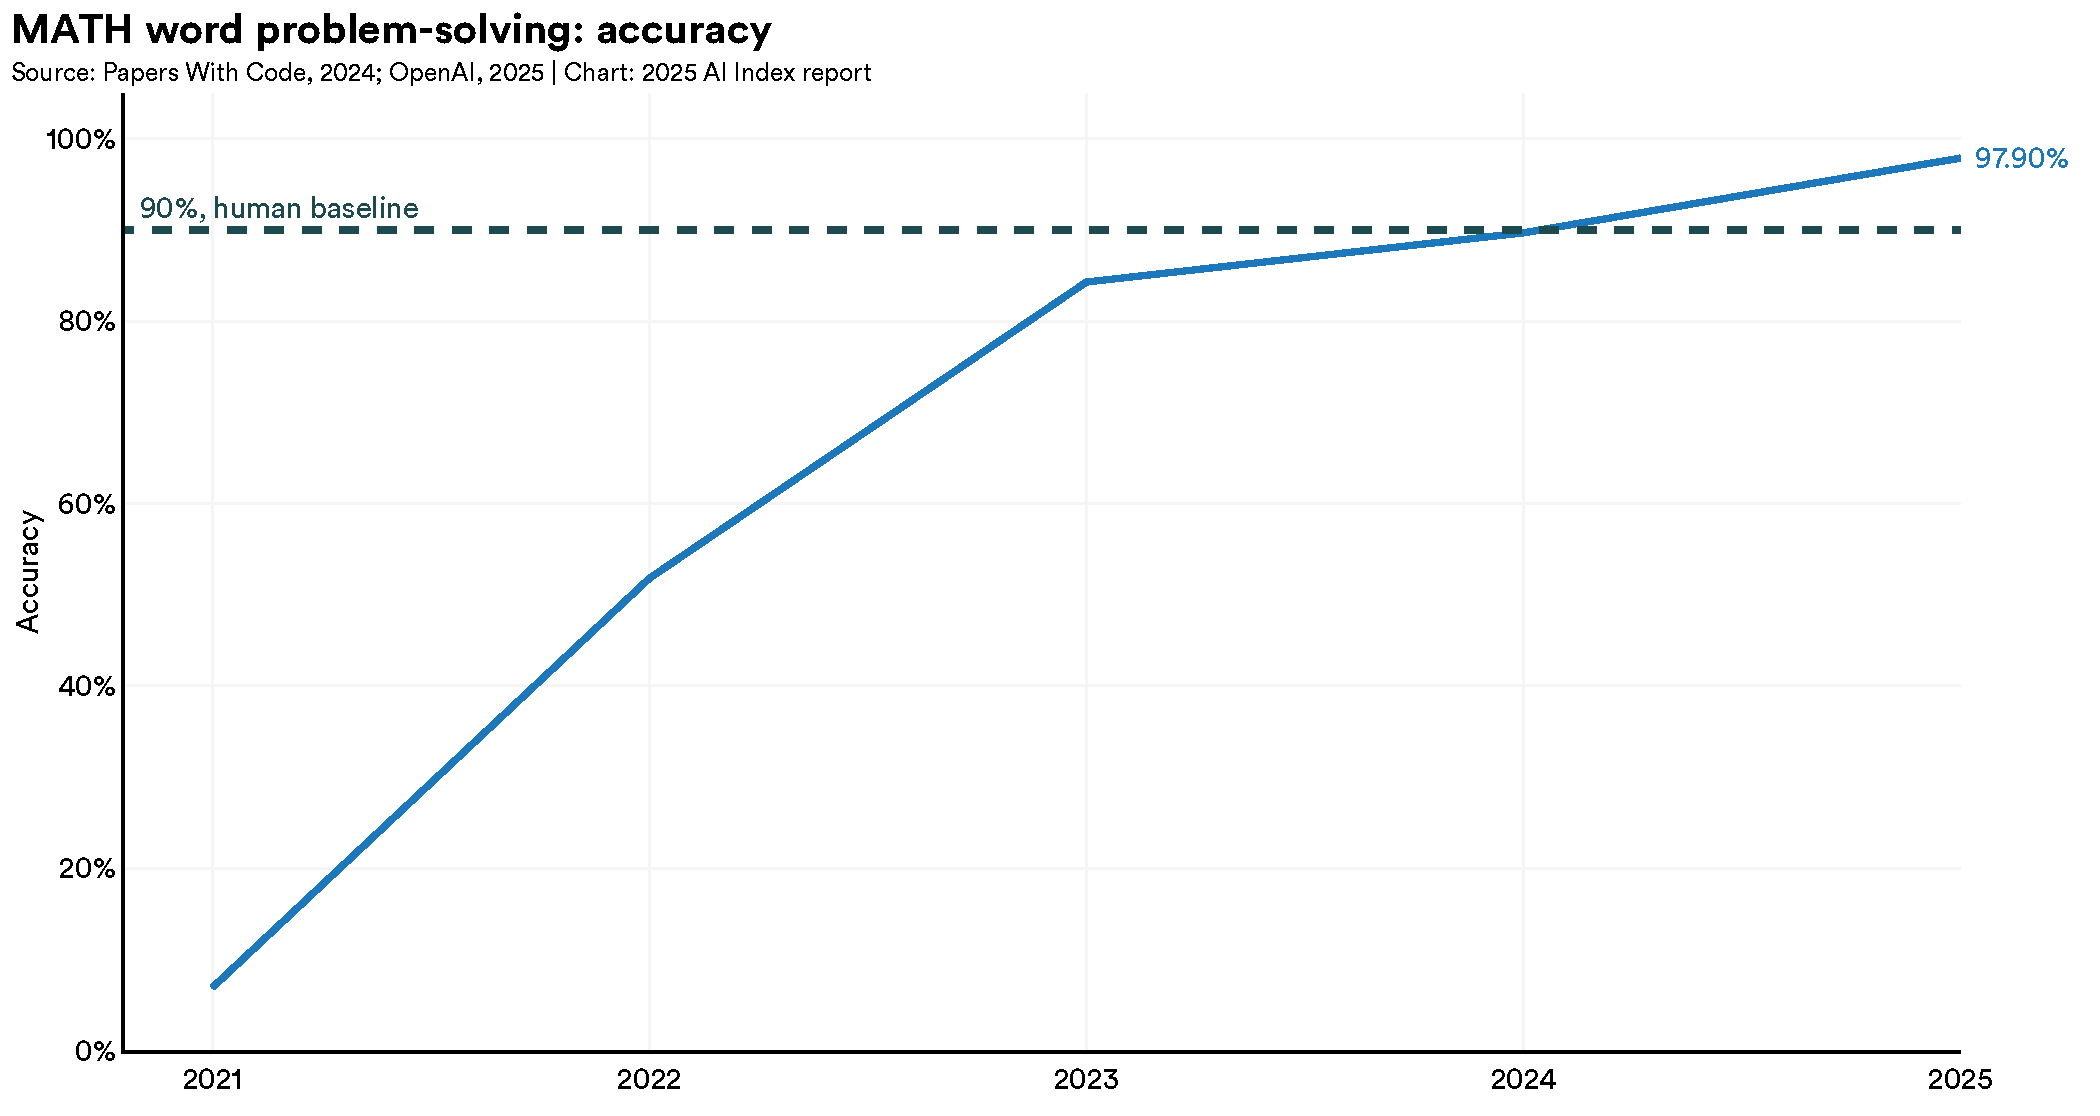
\includegraphics[width=\linewidth]{figures/fig_2.6.4}
		\caption{AI Index Report \url{https://hai.stanford.edu/ai-index/2025-ai-index-report}}
		\label{fig:fig6}
	\end{figure}
\end{frame}

\begin{frame}{Chatbot Arena (Matemáticas)}
	\begin{figure}
		\centering
		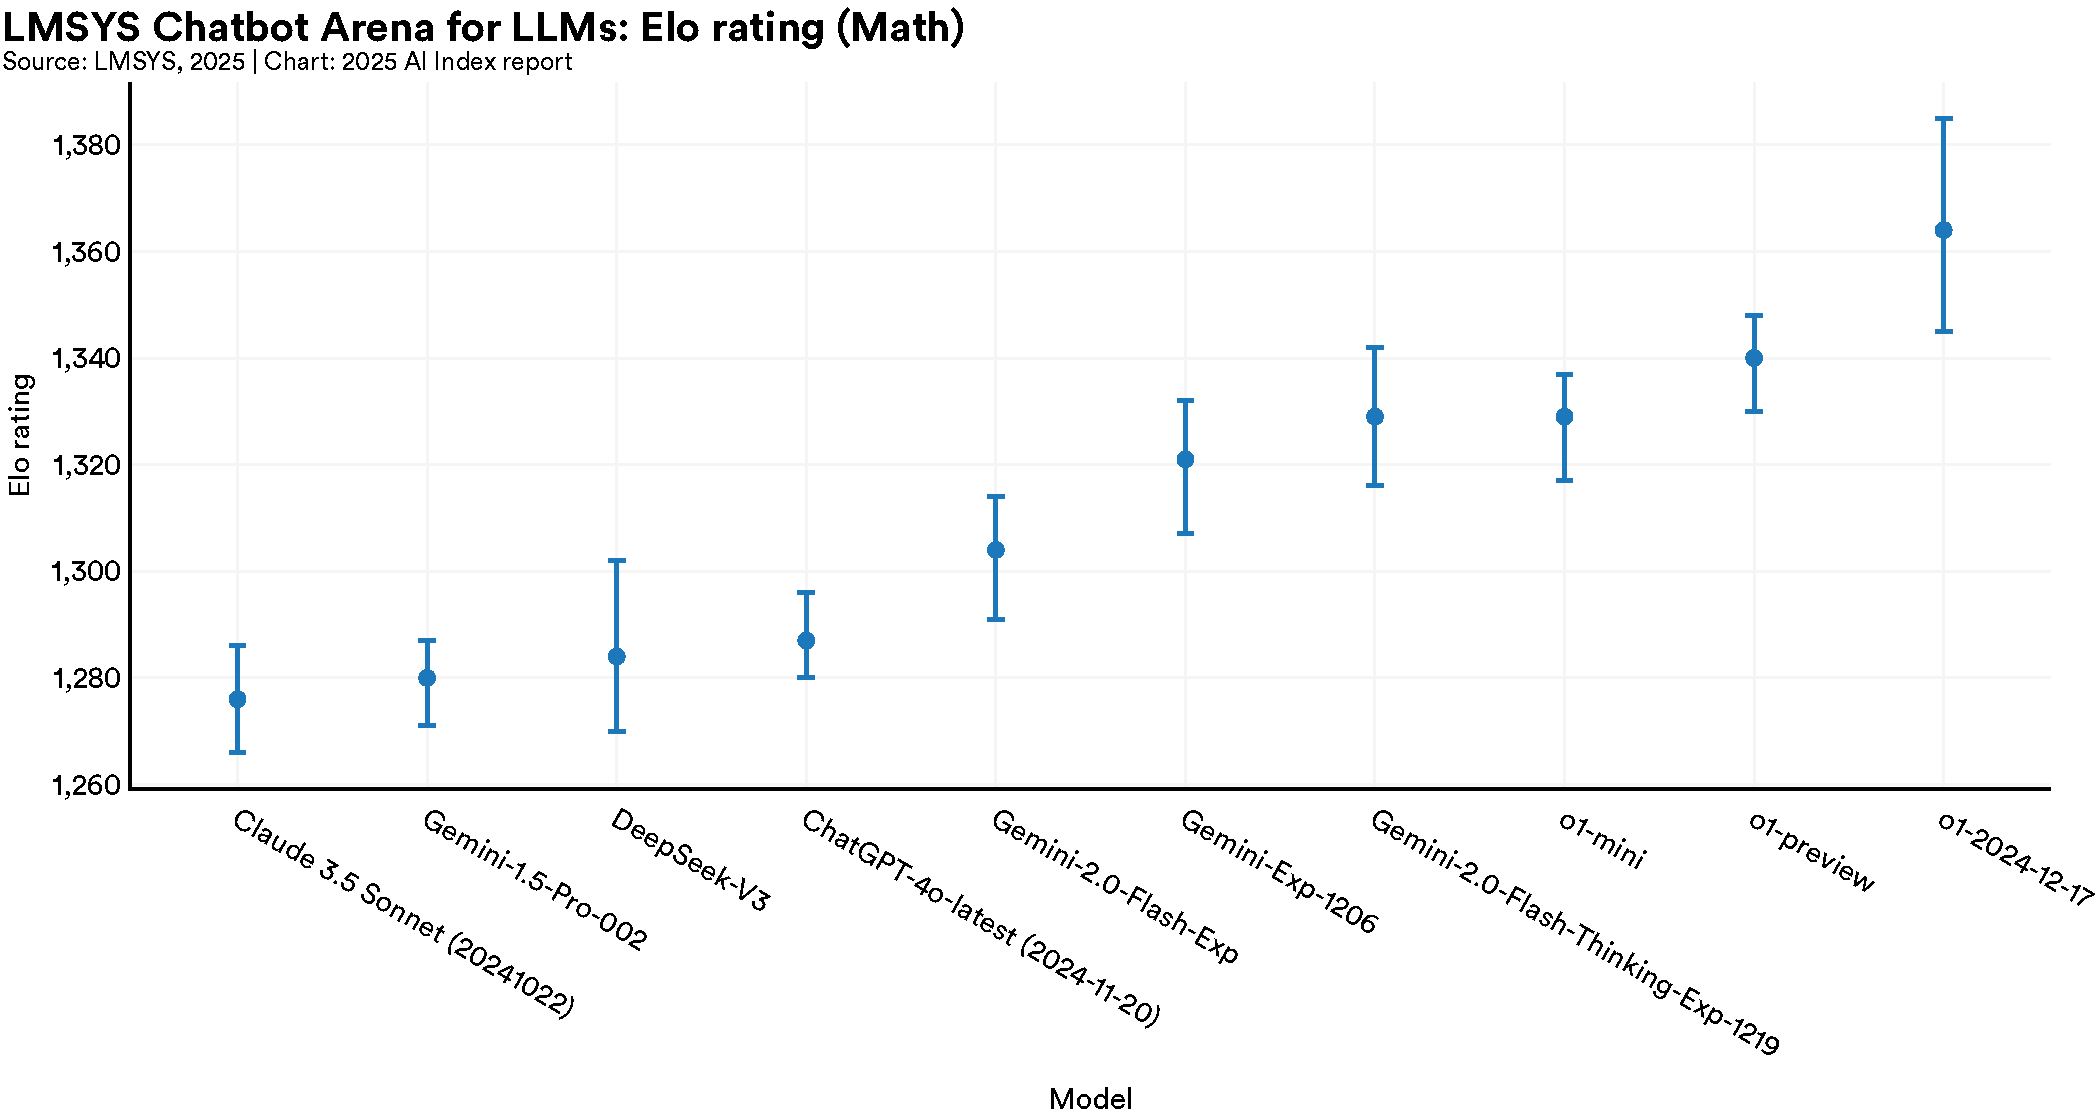
\includegraphics[width=\linewidth]{figures/fig_2.6.5}
		\caption{AI Index Report \url{https://hai.stanford.edu/ai-index/2025-ai-index-report}}
		\label{fig:fig7}
	\end{figure}
\end{frame}

\begin{frame}{Razonamiento}
	\begin{figure}
		\centering
		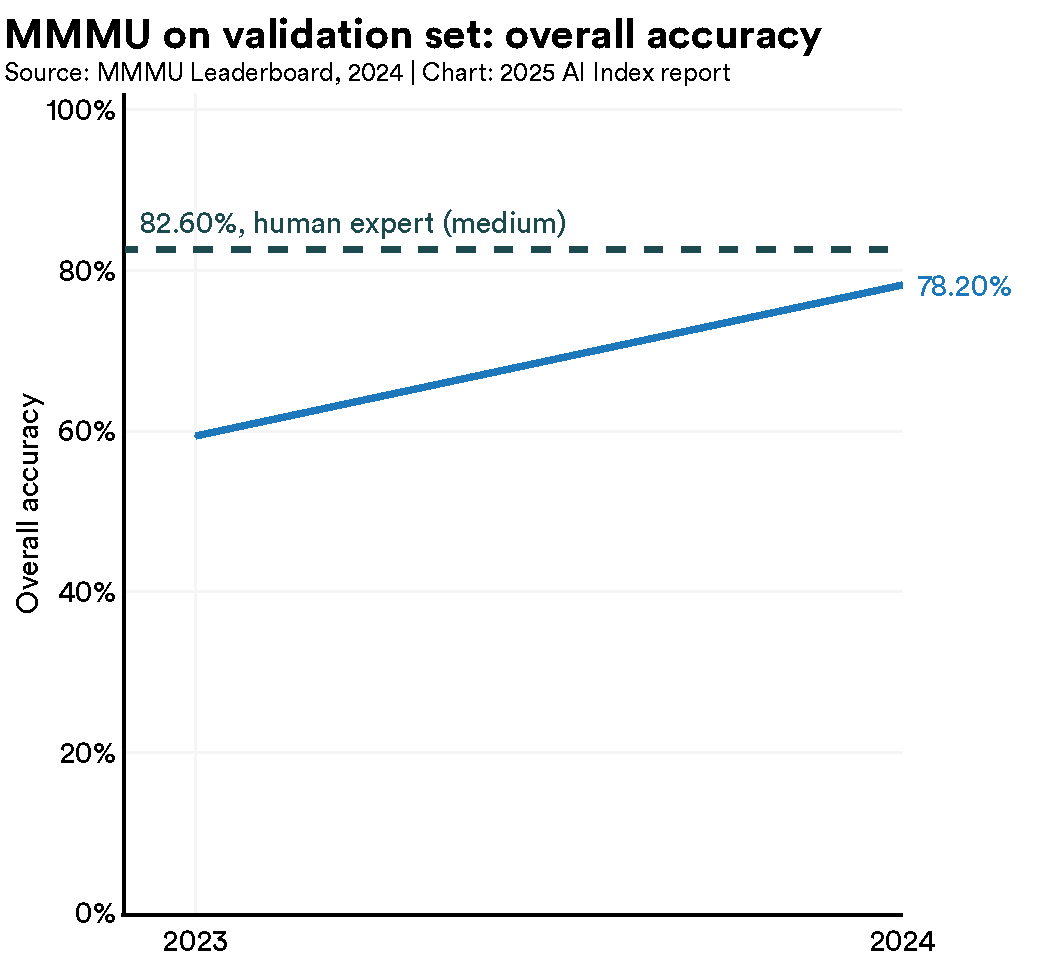
\includegraphics[width=0.6\linewidth]{figures/fig_2.7.2}
		\caption{AI Index Report \url{https://hai.stanford.edu/ai-index/2025-ai-index-report}}
		\label{fig:fig8}
	\end{figure}
\end{frame}

\begin{frame}{Agentes}
	\begin{figure}
		\centering
		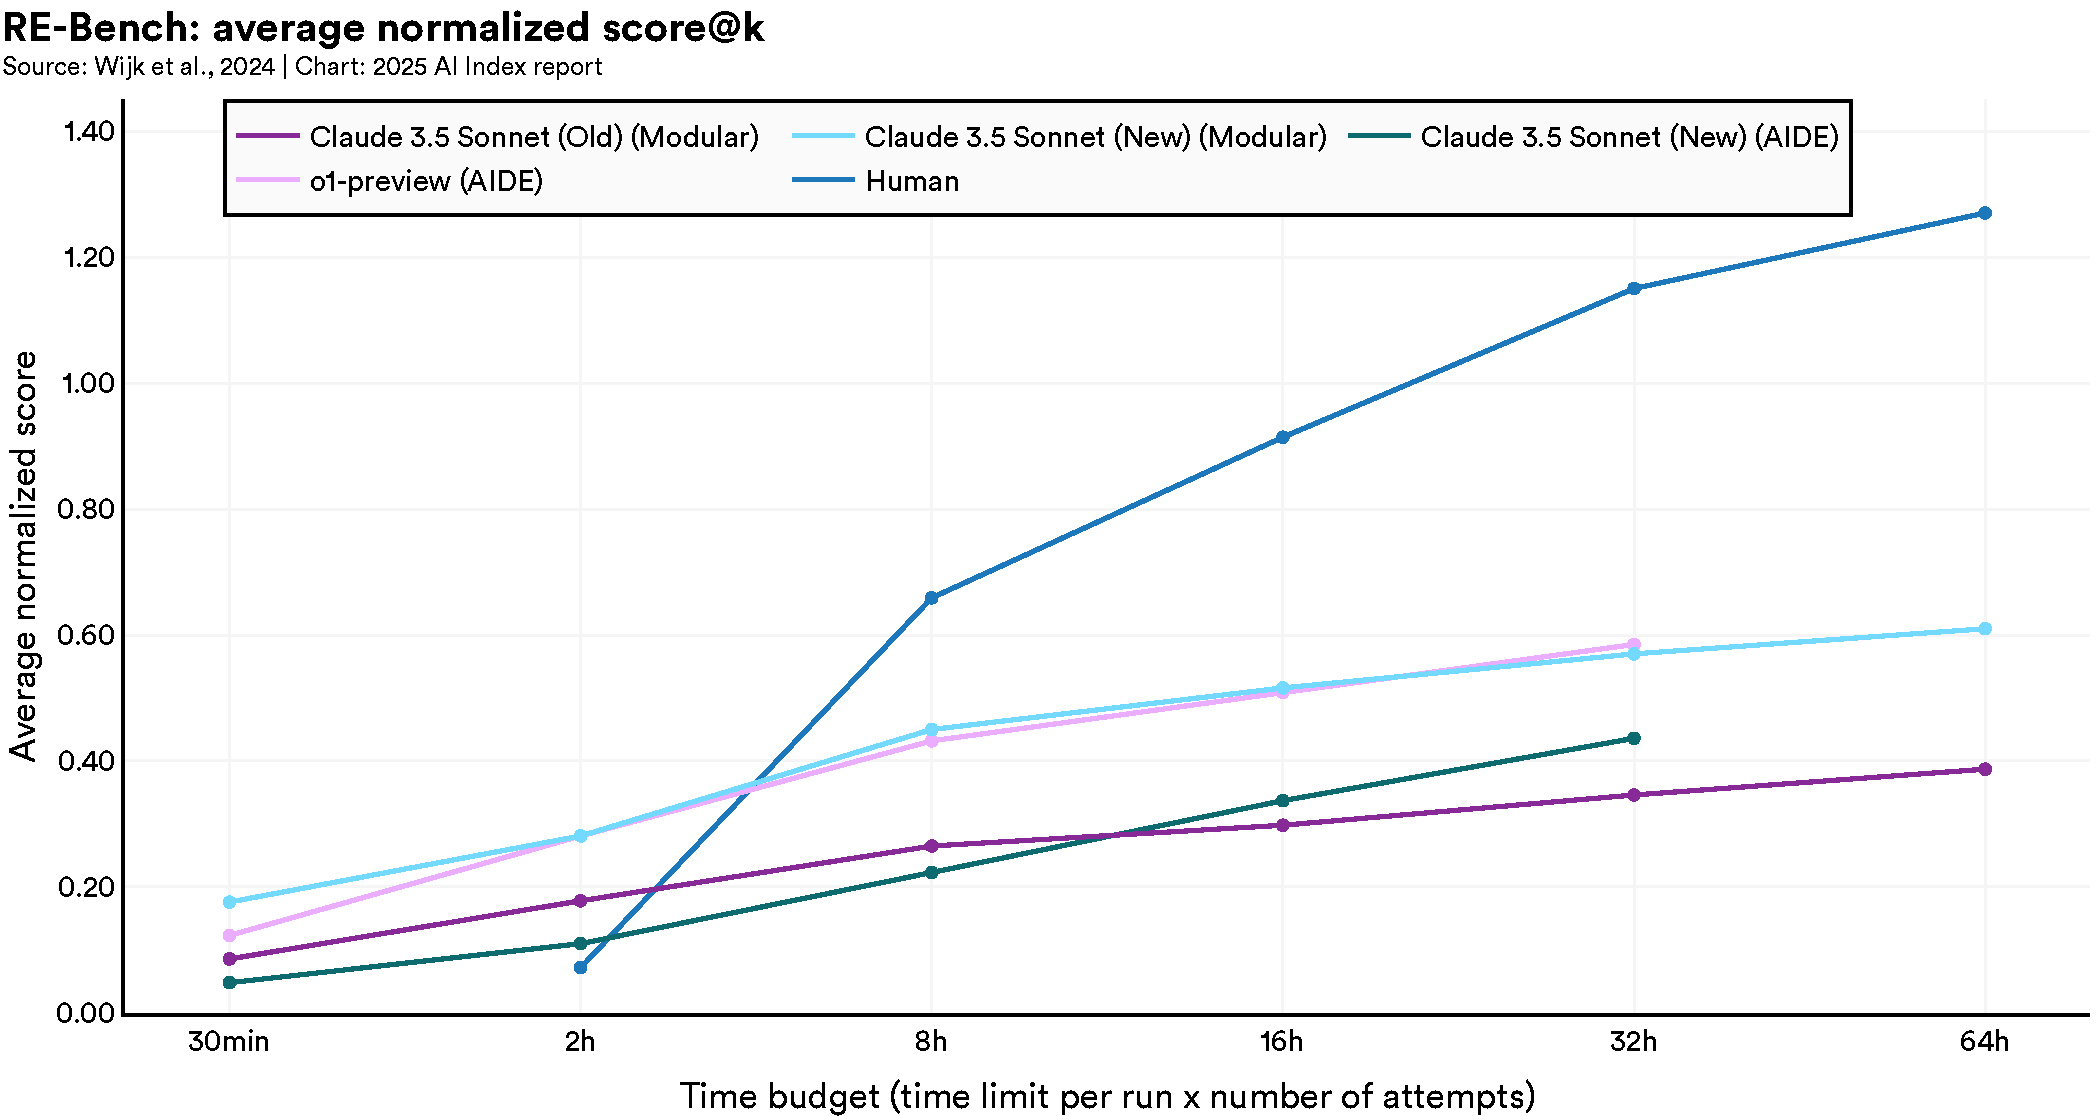
\includegraphics[width=\linewidth]{figures/fig_2.8.4}
		\caption{AI Index Report \url{https://hai.stanford.edu/ai-index/2025-ai-index-report}}
		\label{fig:fig9}
	\end{figure}
\end{frame}

%% --- Diapositiva 8: La Ética en la IA: Un Desafío Crucial ---
\begin{frame}{La Ética en la IA}
  Como científicos de datos, no solo creamos modelos, sino que impactamos a la sociedad. Es imperativo considerar las implicaciones éticas.
  
  \begin{columns}[T]
    \begin{column}{.5\textwidth}
        \begin{alertblock}{Sesgos (Bias)}
            Los modelos aprenden los sesgos presentes en los datos de entrenamiento.
            \begin{itemize}
                \item Sesgo de género en contrataciones.
                \item Sesgo racial en reconocimiento facial.
            \end{itemize}
        \end{alertblock}
        

    \end{column}
    \begin{column}{.5\textwidth}
        \begin{block}{Transparencia y Explicabilidad (XAI)}
            ¿Por qué un modelo tomó una decisión específica?
            \begin{itemize}
                \item Crítico en medicina, finanzas, justicia.
                \item Los modelos de "caja negra" (Deep Learning) son un gran desafío.
            \end{itemize}
        \end{block}
        

    \end{column}
  \end{columns}
\end{frame}

\begin{frame}{La Ética en la IA}
	Como científicos de datos, no solo creamos modelos, sino que impactamos a la sociedad. Es imperativo considerar las implicaciones éticas.
	
	\begin{columns}[T]
		\begin{column}{.5\textwidth}
		
			\begin{exampleblock}{Privacidad}
				Los modelos de IA, especialmente los LLMs, pueden memorizar y filtrar datos sensibles.
				\begin{itemize}
					\item Riesgo de fuga de información personal.
				\end{itemize}
			\end{exampleblock}
		\end{column}
		\begin{column}{.5\textwidth}
			
			\begin{block}{Responsabilidad}
				¿Quién es responsable si un sistema de IA comete un error grave?
				\begin{itemize}
					\item ¿El desarrollador? ¿El usuario? ¿La empresa?
				\end{itemize}
			\end{block}
		\end{column}
	\end{columns}
\end{frame}


%% --- Diapositiva 10: Conclusiones y Preguntas ---
\begin{frame}{Conclusiones}
  \begin{block}{Resumen}
    \begin{itemize}
        \item La IA es un campo vasto y multidisciplinario con una rica historia de ciclos de éxito y desilusión.
        \item Hemos pasado de un enfoque basado en reglas (simbólico) a uno basado en datos (conexionista/ML).
        \item El Deep Learning es la tecnología que impulsa la revolución actual de la IA.
        \item Las consideraciones éticas son tan importantes como la destreza técnica.
    \end{itemize}
  \end{block}

  
\end{frame}

\end{document}